\chapter{Nuclear Engineering Background}
\label{cha:engineering}

\section{Advanced Gas-cooled Reactors (AGRs)} \label{AGR}

The UK nuclear power sector is dominated by the advanced gas-cooled reactor  (AGR) \cite{nonbol1996description}. There are 14 AGR reactors spread across 7 UK power stations . This design differs from most reactors around the world in that it consists of a graphite core cooled by carbon dioxide gas (as opposed to the common water cooled reactor). The international novelty of this design means that all safety analysis has to be performed domestically, leading to a significant requirement for computation.

\begin{figure}[ht!]
	\centering
	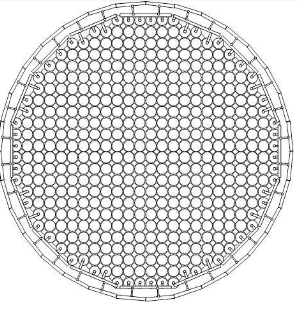
\includegraphics[scale=0.75]{Figures/AGR_plan.png}
	\caption{AGR Core Plan View}
	\label{fig:schematic}
\end{figure}

\noindent
The AGR consists of several thousand stacked graphite bricks assembled in an interlocking 3-dimensional assembly (shown in Figure~\ref{fig:schematic} and \ref{fig:side}). There are two principal brick types shown in Figure~\ref{fig:bricks}: (1) large bore bricks for the insertion of fuel assemblies and (2) interstitial bricks which provide structural support, some of which have a small bore to allow the insertion of a control rod. The bricks are linked and held in position by rectangular graphite keys. An individual stack of bricks the height of the core is known as a channel, with types of channel dictated by the type of brick i.e. fuel, control rod, filler, peripheral (fuel channels near the edge of the core) and reflector (the shape of fuel bricks but contain no fuel and are solid) channels. 

\begin{figure}[ht!]
	\centering
	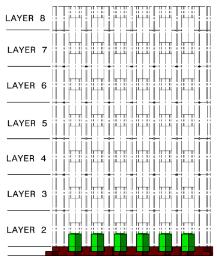
\includegraphics[scale=0.75]{Figures/AGR_side}
	\caption{AGR Core Side View}
	\label{fig:side}
\end{figure}

\noindent
The primary safety concern with the AGR is the cracking of the fuel bricks. Given enough cracks, the ability to insert fuel or control rods could be impeded. The mechanism by which the cracks occur is well understood. The intense heat and radiation cause a reduction in the mass and volume of the bricks, resulting in a stress differential, which leads to a concentration of stress and cracking at the root of the keyways (Figure \ref{fig:cracking}). \\ 

\noindent
The growth of these cracks ultimately results in the splitting of the brick into two halves (see Figure \ref{fig:cracked}). At any given time, it is difficult to ascertain which bricks are exhibiting cracks due to inaccessible nature of the core internals. Forecasting the location of cracks as a function of time is an area of ongoing research. Future inspection regimes may yield better information about where cracks are occurring.

\section{Traditional Engineering Safety Assessments} \label{Engineering}
The UK Office for Nuclear Regulation (ONR) stipulates that the AGR operator (EDF Energy) must demonstrate that the ability to control the reactor (i.e. insert control rods) will not be threatened under any circumstance i.e an earthquake or other serious event.\\

\begin{figure}[ht!]
	\centering
	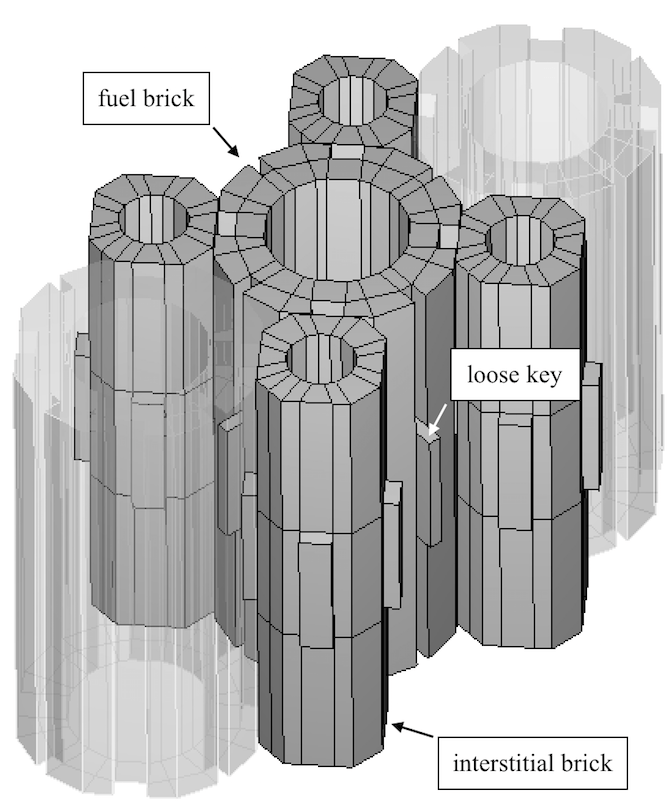
\includegraphics[scale=0.17]{Figures/brick_types_parmec}
	\caption{AGR Core Brick Types}
	\label{fig:bricks}
\end{figure}

\begin{figure}[ht!]
	\centering
	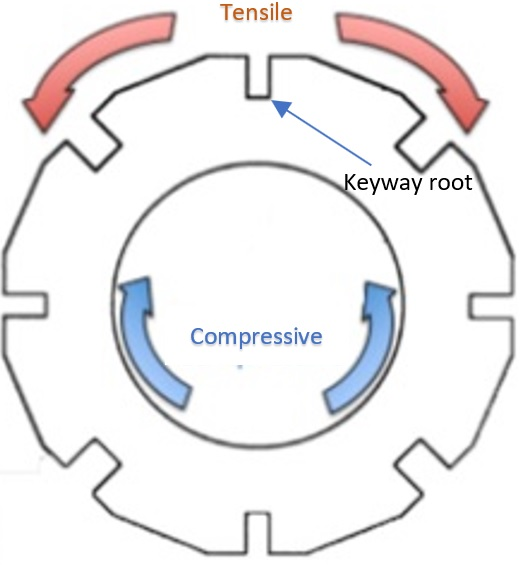
\includegraphics[scale=0.35]{Figures/cracking_mechanism}
	\caption{Brick Cracking Mechanism}
	\label{fig:cracking}
\end{figure}

\begin{figure}[ht!]
	\centering
	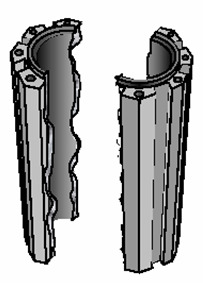
\includegraphics[scale=0.65]{Figures/Brick_Cracking}
	\caption{Cracked AGR Brick}
	\label{fig:cracked}
\end{figure}

\begin{figure}[b!]
	\centering
	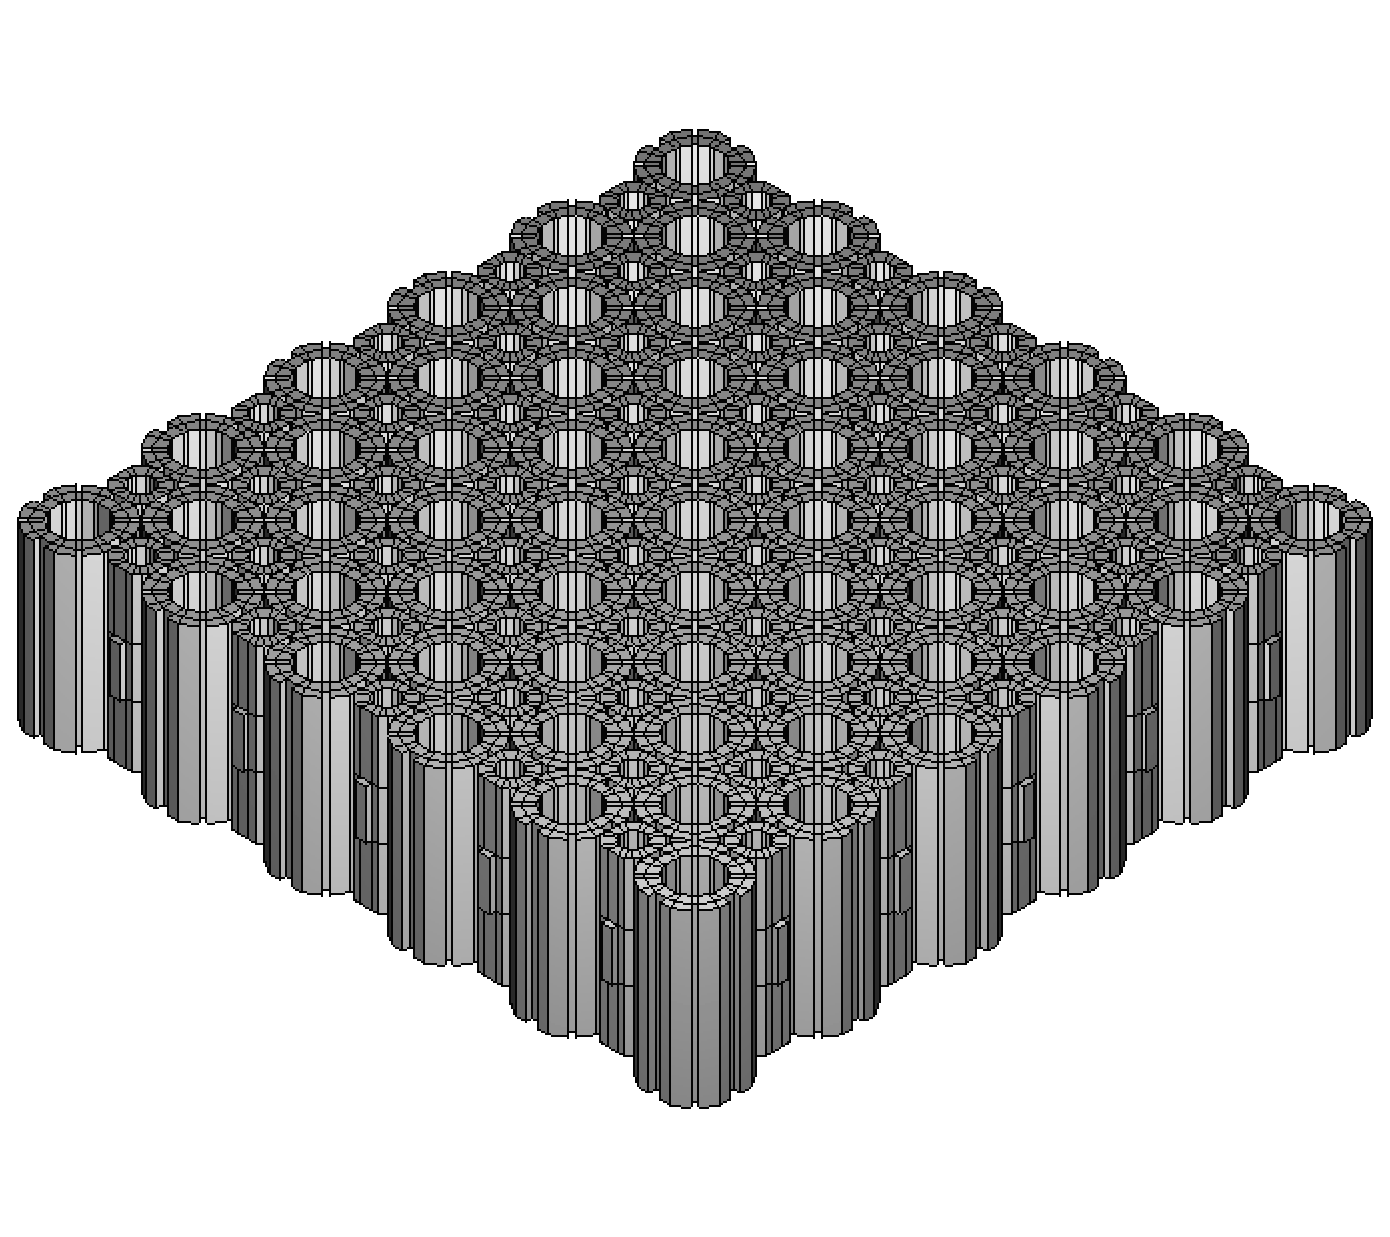
\includegraphics[scale=0.12]{Figures/parmec_bricks.png}
	\caption{Visualisation of Parmec Model}
	\label{fig:FEA}
\end{figure}

\noindent
The traditional approach used to ensure the safe condition of the AGR involves production and analysis of complex engineering models, which are deterministic and rely on physical relationships. Examples include the computational model Parmec \cite{wiki:xxx} and the physical Multi-Layer Array (MLA) model \cite{dihoru2014multi} at the University of Bristol (Figures \ref{fig:FEA} \& \ref{fig:ENG}, respectively). Both of these models are configured to to simulate a once in 10,000 year earthquake. \\

\begin{figure}[b!]
	\centering
	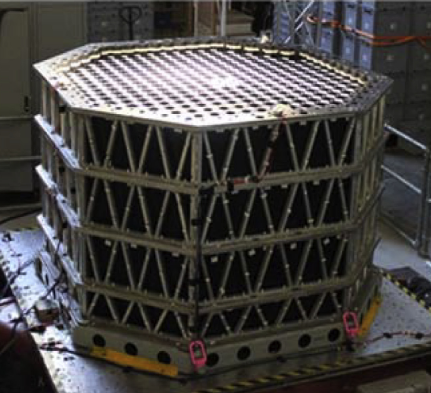
\includegraphics[scale=0.5]{Figures/MLA_rig}
	\caption{Multi-Layer Array Rig}
	\label{fig:ENG}
\end{figure}

\noindent
As mentioned at the end of section~\ref{AGR}, it is difficult to ascertain where the cracks are (or where they will occur). In lieu of actual crack positions, the traditional approach is to generate a random distribution of cracks, represented by a 3-dimensional array as shown in Figure~\ref{fig:core_array}. This array constitutes the structure of the AGR core, with the position of each element corresponding to a spatial position of a brick. This array has an integer data-type: -1 is an intact brick, 0 represents a reflector brick and 1~-~4 representing crack orientations - see Figure~\ref{fig:orientations}. \\

\begin{figure}[ht!]
	\centering
	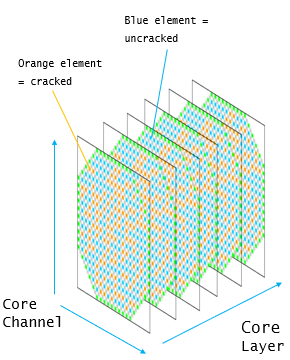
\includegraphics[scale=0.5]{Figures/core_array.png}
	\caption{AGR Input Core Array}
	\label{fig:core_array}
\end{figure}

\begin{figure}[ht!]
	\centering
	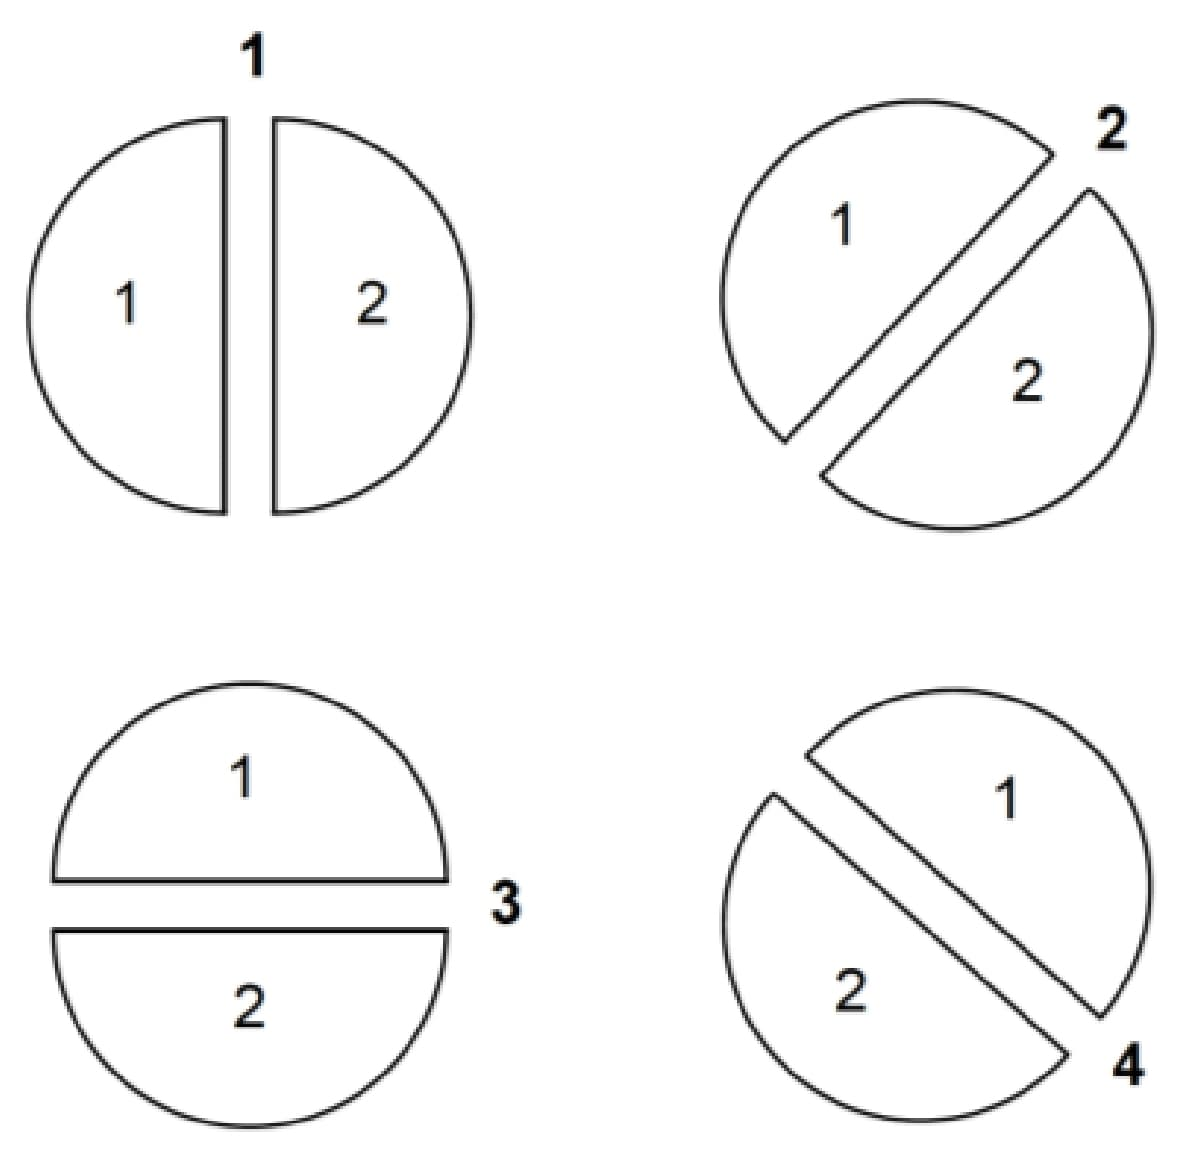
\includegraphics[scale=0.1]{Figures/orientations}
	\caption{Brick Crack Orientations}
	\label{fig:orientations}
\end{figure}

\noindent
The example array shown in Figure~\ref{fig:core_array} can be generated quickly and with low computational cost using industry standard tools (usually less than 1 minute per instance). These arrays can be used as input configurations to engineering models such as those shown in Figure~\ref{fig:FEA}~or~Figure~\ref{fig:ENG}. \\

\begin{figure}[ht!]
	\centering
	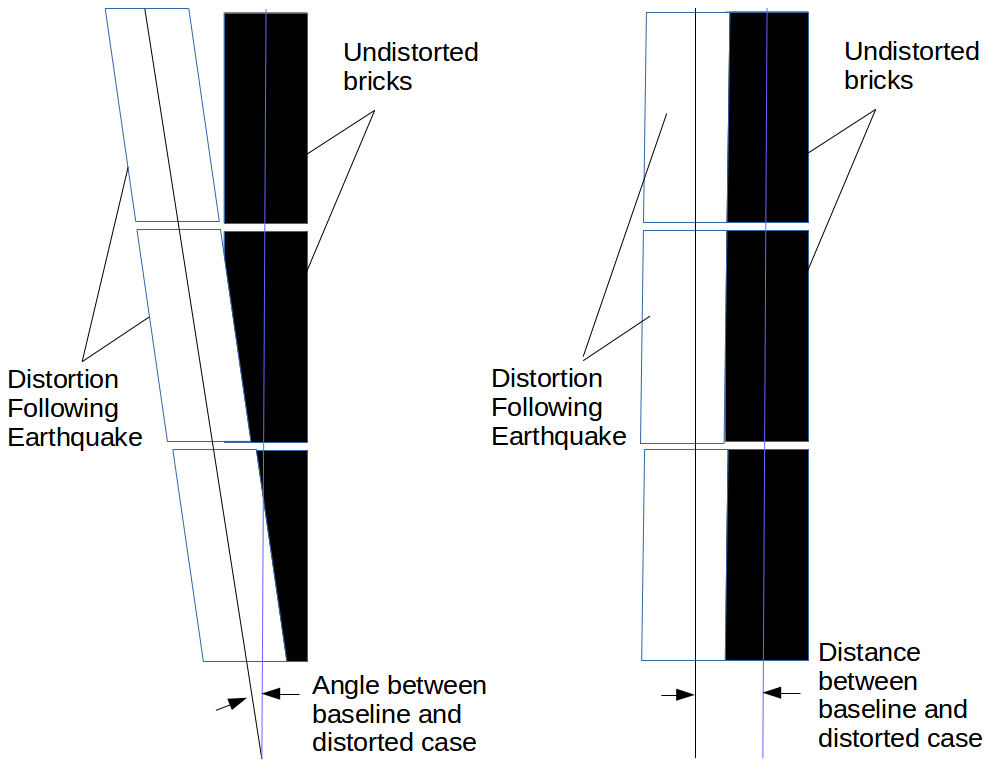
\includegraphics[scale=0.2]{Figures/Distored_bricks}
	\caption{Angle Between a Distorted and Baseline Brick Channel }
	\label{fig:angles}
\end{figure}

% 2D array
% Statistical Analysis

\noindent
The models are able to calculate the position of the bricks following an earthquake (Figure~\ref{fig:angles}) with the presence of cracked bricks influencing how the they move. Angular or translational movement of the bricks acts to effectively reduce the clearance between the fuel or control rod and the surrounding bore wall. Figure~\ref{fig:bore_clearance} illustrates an example involving a control rod channel: the relative displacement of the control rod insertion point can be calculated as a function of the movement of the bricks. The path of the control rod must not be obstructed, and so the relative displacement must be less than the bore radius. \\

\begin{figure}[ht!]
	\centering
	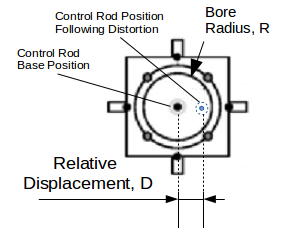
\includegraphics[scale=0.5]{Figures/bore_displacement}
	\caption{Relative Displacement of Control Rod}
	\label{fig:bore_clearance}
\end{figure}

\noindent
The outputs shown in Figures~\ref{fig:angles} \& \ref{fig:bore_clearance} are calculated for every vertical channel. This may include all control rod and/or fuel channels and so can be represented by a 2D array as shown in Figure~\ref{fig:output_array}.\\

\begin{figure}[ht!]
	\centering
	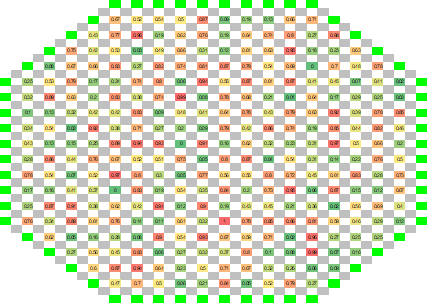
\includegraphics[scale=0.4]{Figures/agr_output.png}
	\caption{AGR Output Core Array}
	\label{fig:output_array}
\end{figure}

\noindent
A single iteration of the aforementioned process, summarised in Figure~\ref{fig:traditional}, gives us very little information on its own. With multiple iterations of this process, each with a different randomised state of the input array (Figure~\ref{fig:core_array}), a stochastic  understanding of the problem space can be built. For example, with several hundred iterations, a histogram can be plotted, as shown in Figure~\ref{fig:statistical_analysis}. The frequency of results is then fitted to a statistical distribution, such as the Normal distribution. Using this distribution, it can be determined what percentage of results are above an acceptable threshold (for instance, half the bore radius shown in \ref{fig:bore_clearance}). Using these statistics, determinations can be made of the probability of certain serious events occurring and are used in safety decision making.\\



\noindent
Both of these engineering modelling methods mentioned in this subsection are expensive in terms of time, computation and/or materials. This expense represents a significant bottleneck to the process summarised in Figure~\ref{fig:traditional}.\\

\noindent
There are also ongoing inspection results to determine the actual positions of cracks. During any inspection interval it is only possible to examine a small number of bricks for cracks. Further, the inspection schedule is infrequent (once every 1 - 3 years) and it is difficult to forecast where new cracks will occur. In the future, improved inspection techniques and better understanding of the process that leads to cracking will yield better information about where and when cracks will occur.

\begin{figure}[b!]
	\centering
	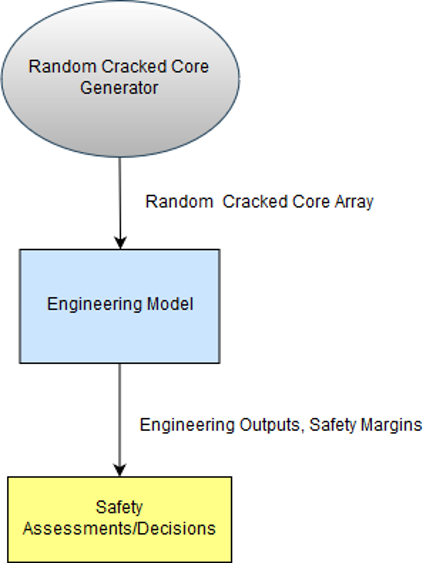
\includegraphics[scale=0.5]{Figures/engineering_approach}
	\caption{Traditional Engineering Approach}
	\label{fig:traditional}
\end{figure}

\begin{figure}[t]
	\centering
	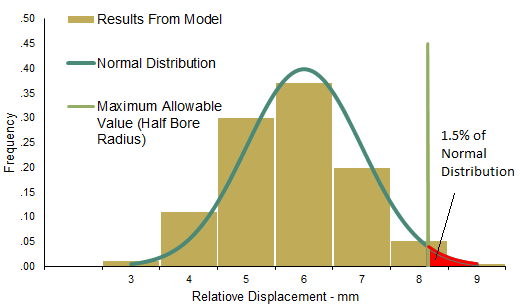
\includegraphics[scale=0.55]{Figures/Statistical_analysis}
	\caption{Statistical Analysis}
	\label{fig:statistical_analysis}
\end{figure}

\section{Relevant Literature}

The AGR reactor and its response to seismic activity is well studied in academic literature. In \cite{voyagaki2018earthquake}, both a computational and experimental examination of the AGR reactor is made. This paper discusses various seismic configurations, all involving an intact core i.e. without cracked bricks. The authors note that without cracking, an obstruction of a control rod channel during a seismic event is not possible due to the design of the core. Elsewhere, \cite{oddbjornsson2017physical} looks at the effects of cracking in a physical AGR experiment at the University of Bristol. The results of this work help validate computational studies. A noteworthy finding is that displacements tend to be greater near the centre of the core.